% Created by tikzDevice version 0.12.3.1 on 2022-10-20 16:36:11
% !TEX encoding = UTF-8 Unicode
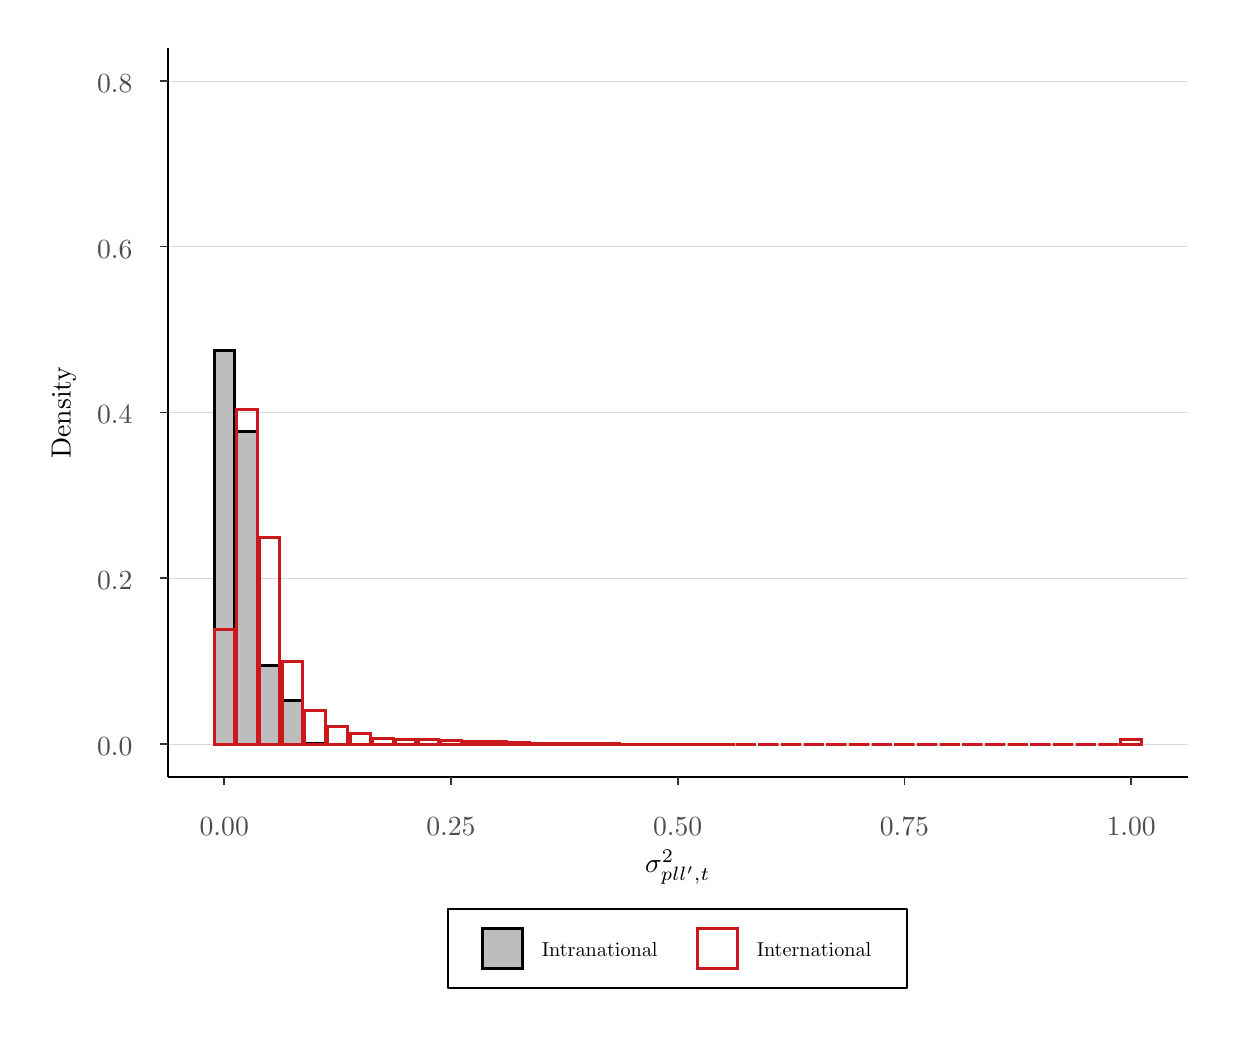
\begin{tikzpicture}[x=1pt,y=1pt]
\definecolor{fillColor}{RGB}{255,255,255}
\path[use as bounding box,fill=fillColor,fill opacity=0.00] (0,0) rectangle (433.62,361.35);
\begin{scope}
\path[clip] (  0.00,  0.00) rectangle (433.62,361.35);
\definecolor{drawColor}{RGB}{255,255,255}
\definecolor{fillColor}{RGB}{255,255,255}

\path[draw=drawColor,line width= 0.6pt,line join=round,line cap=round,fill=fillColor] (  0.00,  0.00) rectangle (433.62,361.35);
\end{scope}
\begin{scope}
\path[clip] ( 50.59, 90.50) rectangle (419.17,354.12);
\definecolor{drawColor}{RGB}{255,255,255}

\path[draw=drawColor,line width= 0.3pt,line join=round] ( 50.59,132.44) --
	(419.17,132.44);

\path[draw=drawColor,line width= 0.3pt,line join=round] ( 50.59,192.35) --
	(419.17,192.35);

\path[draw=drawColor,line width= 0.3pt,line join=round] ( 50.59,252.27) --
	(419.17,252.27);

\path[draw=drawColor,line width= 0.3pt,line join=round] ( 50.59,312.18) --
	(419.17,312.18);

\path[draw=drawColor,line width= 0.3pt,line join=round] (111.99, 90.50) --
	(111.99,354.12);

\path[draw=drawColor,line width= 0.3pt,line join=round] (193.92, 90.50) --
	(193.92,354.12);

\path[draw=drawColor,line width= 0.3pt,line join=round] (275.84, 90.50) --
	(275.84,354.12);

\path[draw=drawColor,line width= 0.3pt,line join=round] (357.76, 90.50) --
	(357.76,354.12);
\definecolor{drawColor}{gray}{0.85}

\path[draw=drawColor,line width= 0.1pt,line join=round] ( 50.59,102.48) --
	(419.17,102.48);

\path[draw=drawColor,line width= 0.1pt,line join=round] ( 50.59,162.40) --
	(419.17,162.40);

\path[draw=drawColor,line width= 0.1pt,line join=round] ( 50.59,222.31) --
	(419.17,222.31);

\path[draw=drawColor,line width= 0.1pt,line join=round] ( 50.59,282.23) --
	(419.17,282.23);

\path[draw=drawColor,line width= 0.1pt,line join=round] ( 50.59,342.14) --
	(419.17,342.14);
\definecolor{drawColor}{RGB}{0,0,0}
\definecolor{fillColor}{gray}{0.74}

\path[draw=drawColor,line width= 1.1pt,line cap=rect,fill=fillColor] ( 67.34,102.48) rectangle ( 74.72,244.76);
\definecolor{drawColor}{RGB}{203,24,29}

\path[draw=drawColor,line width= 1.1pt,line cap=rect] ( 67.34,102.48) rectangle ( 74.72,143.84);
\definecolor{drawColor}{RGB}{0,0,0}

\path[draw=drawColor,line width= 1.1pt,line cap=rect,fill=fillColor] ( 75.54,102.48) rectangle ( 82.91,215.42);
\definecolor{drawColor}{RGB}{203,24,29}

\path[draw=drawColor,line width= 1.1pt,line cap=rect] ( 75.54,102.48) rectangle ( 82.91,223.26);
\definecolor{drawColor}{RGB}{0,0,0}

\path[draw=drawColor,line width= 1.1pt,line cap=rect,fill=fillColor] ( 83.73,102.48) rectangle ( 91.10,130.82);
\definecolor{drawColor}{RGB}{203,24,29}

\path[draw=drawColor,line width= 1.1pt,line cap=rect] ( 83.73,102.48) rectangle ( 91.10,177.11);
\definecolor{drawColor}{RGB}{0,0,0}

\path[draw=drawColor,line width= 1.1pt,line cap=rect,fill=fillColor] ( 91.92,102.48) rectangle ( 99.29,118.12);
\definecolor{drawColor}{RGB}{203,24,29}

\path[draw=drawColor,line width= 1.1pt,line cap=rect] ( 91.92,102.48) rectangle ( 99.29,132.47);
\definecolor{drawColor}{RGB}{0,0,0}

\path[draw=drawColor,line width= 1.1pt,line cap=rect,fill=fillColor] (100.11,102.48) rectangle (107.49,102.85);
\definecolor{drawColor}{RGB}{203,24,29}

\path[draw=drawColor,line width= 1.1pt,line cap=rect] (100.11,102.48) rectangle (107.49,114.61);
\definecolor{drawColor}{RGB}{0,0,0}

\path[draw=drawColor,line width= 1.1pt,line cap=rect,fill=fillColor] (108.31,102.48) rectangle (115.68,102.49);
\definecolor{drawColor}{RGB}{203,24,29}

\path[draw=drawColor,line width= 1.1pt,line cap=rect] (108.31,102.48) rectangle (115.68,108.95);
\definecolor{drawColor}{RGB}{0,0,0}

\path[draw=drawColor,line width= 1.1pt,line cap=rect,fill=fillColor] (116.50,102.48) rectangle (123.87,102.48);
\definecolor{drawColor}{RGB}{203,24,29}

\path[draw=drawColor,line width= 1.1pt,line cap=rect] (116.50,102.48) rectangle (123.87,106.15);
\definecolor{drawColor}{RGB}{0,0,0}

\path[draw=drawColor,line width= 1.1pt,line cap=rect,fill=fillColor] (124.69,102.48) rectangle (132.06,102.48);
\definecolor{drawColor}{RGB}{203,24,29}

\path[draw=drawColor,line width= 1.1pt,line cap=rect] (124.69,102.48) rectangle (132.06,104.38);
\definecolor{drawColor}{RGB}{0,0,0}

\path[draw=drawColor,line width= 1.1pt,line cap=rect,fill=fillColor] (132.88,102.48) rectangle (140.26,102.48);
\definecolor{drawColor}{RGB}{203,24,29}

\path[draw=drawColor,line width= 1.1pt,line cap=rect] (132.88,102.48) rectangle (140.26,104.01);
\definecolor{drawColor}{RGB}{0,0,0}

\path[draw=drawColor,line width= 1.1pt,line cap=rect,fill=fillColor] (141.08,102.48) rectangle (148.45,102.48);
\definecolor{drawColor}{RGB}{203,24,29}

\path[draw=drawColor,line width= 1.1pt,line cap=rect] (141.08,102.48) rectangle (148.45,104.07);
\definecolor{drawColor}{RGB}{0,0,0}

\path[draw=drawColor,line width= 1.1pt,line cap=rect,fill=fillColor] (149.27,102.48) rectangle (156.64,102.48);
\definecolor{drawColor}{RGB}{203,24,29}

\path[draw=drawColor,line width= 1.1pt,line cap=rect] (149.27,102.48) rectangle (156.64,103.75);
\definecolor{drawColor}{RGB}{0,0,0}

\path[draw=drawColor,line width= 1.1pt,line cap=rect,fill=fillColor] (157.46,102.48) rectangle (164.83,102.48);
\definecolor{drawColor}{RGB}{203,24,29}

\path[draw=drawColor,line width= 1.1pt,line cap=rect] (157.46,102.48) rectangle (164.83,103.40);
\definecolor{drawColor}{RGB}{0,0,0}

\path[draw=drawColor,line width= 1.1pt,line cap=rect,fill=fillColor] (165.65,102.48) rectangle (173.03,102.48);
\definecolor{drawColor}{RGB}{203,24,29}

\path[draw=drawColor,line width= 1.1pt,line cap=rect] (165.65,102.48) rectangle (173.03,103.28);
\definecolor{drawColor}{RGB}{0,0,0}

\path[draw=drawColor,line width= 1.1pt,line cap=rect,fill=fillColor] (173.85,102.48) rectangle (181.22,102.48);
\definecolor{drawColor}{RGB}{203,24,29}

\path[draw=drawColor,line width= 1.1pt,line cap=rect] (173.85,102.48) rectangle (181.22,103.03);

\path[draw=drawColor,line width= 1.1pt,line cap=rect] (182.04,102.48) rectangle (189.41,102.71);
\definecolor{drawColor}{RGB}{0,0,0}

\path[draw=drawColor,line width= 1.1pt,line cap=rect,fill=fillColor] (190.23,102.48) rectangle (197.60,102.48);
\definecolor{drawColor}{RGB}{203,24,29}

\path[draw=drawColor,line width= 1.1pt,line cap=rect] (190.23,102.48) rectangle (197.60,102.55);

\path[draw=drawColor,line width= 1.1pt,line cap=rect] (198.42,102.48) rectangle (205.80,102.52);
\definecolor{drawColor}{RGB}{0,0,0}

\path[draw=drawColor,line width= 1.1pt,line cap=rect,fill=fillColor] (206.61,102.48) rectangle (213.99,102.48);
\definecolor{drawColor}{RGB}{203,24,29}

\path[draw=drawColor,line width= 1.1pt,line cap=rect] (206.61,102.48) rectangle (213.99,102.50);
\definecolor{drawColor}{RGB}{0,0,0}

\path[draw=drawColor,line width= 1.1pt,line cap=rect,fill=fillColor] (214.81,102.48) rectangle (222.18,102.48);
\definecolor{drawColor}{RGB}{203,24,29}

\path[draw=drawColor,line width= 1.1pt,line cap=rect] (214.81,102.48) rectangle (222.18,102.49);

\path[draw=drawColor,line width= 1.1pt,line cap=rect] (223.00,102.48) rectangle (230.37,102.49);

\path[draw=drawColor,line width= 1.1pt,line cap=rect] (231.19,102.48) rectangle (238.56,102.49);
\definecolor{drawColor}{RGB}{0,0,0}

\path[draw=drawColor,line width= 1.1pt,line cap=rect,fill=fillColor] (239.38,102.48) rectangle (246.76,102.48);
\definecolor{drawColor}{RGB}{203,24,29}

\path[draw=drawColor,line width= 1.1pt,line cap=rect] (239.38,102.48) rectangle (246.76,102.49);

\path[draw=drawColor,line width= 1.1pt,line cap=rect] (247.58,102.48) rectangle (254.95,102.49);

\path[draw=drawColor,line width= 1.1pt,line cap=rect] (255.77,102.48) rectangle (263.14,102.48);

\path[draw=drawColor,line width= 1.1pt,line cap=rect] (263.96,102.48) rectangle (271.33,102.48);

\path[draw=drawColor,line width= 1.1pt,line cap=rect] (272.15,102.48) rectangle (279.53,102.48);

\path[draw=drawColor,line width= 1.1pt,line cap=rect] (280.35,102.48) rectangle (287.72,102.48);

\path[draw=drawColor,line width= 1.1pt,line cap=rect] (288.54,102.48) rectangle (295.91,102.48);

\path[draw=drawColor,line width= 1.1pt,line cap=rect] (296.73,102.48) rectangle (304.10,102.48);

\path[draw=drawColor,line width= 1.1pt,line cap=rect] (304.92,102.48) rectangle (312.30,102.48);

\path[draw=drawColor,line width= 1.1pt,line cap=rect] (313.12,102.48) rectangle (320.49,102.48);

\path[draw=drawColor,line width= 1.1pt,line cap=rect] (321.31,102.48) rectangle (328.68,102.48);

\path[draw=drawColor,line width= 1.1pt,line cap=rect] (329.50,102.48) rectangle (336.87,102.48);

\path[draw=drawColor,line width= 1.1pt,line cap=rect] (337.69,102.48) rectangle (345.07,102.48);

\path[draw=drawColor,line width= 1.1pt,line cap=rect] (345.89,102.48) rectangle (353.26,102.48);

\path[draw=drawColor,line width= 1.1pt,line cap=rect] (354.08,102.48) rectangle (361.45,102.48);

\path[draw=drawColor,line width= 1.1pt,line cap=rect] (362.27,102.48) rectangle (369.64,102.48);

\path[draw=drawColor,line width= 1.1pt,line cap=rect] (370.46,102.48) rectangle (377.84,102.48);

\path[draw=drawColor,line width= 1.1pt,line cap=rect] (378.65,102.48) rectangle (386.03,102.48);

\path[draw=drawColor,line width= 1.1pt,line cap=rect] (386.85,102.48) rectangle (394.22,102.48);
\definecolor{drawColor}{RGB}{0,0,0}

\path[draw=drawColor,line width= 1.1pt,line cap=rect,fill=fillColor] (395.04,102.48) rectangle (402.41,102.48);
\definecolor{drawColor}{RGB}{203,24,29}

\path[draw=drawColor,line width= 1.1pt,line cap=rect] (395.04,102.48) rectangle (402.41,104.09);
\end{scope}
\begin{scope}
\path[clip] (  0.00,  0.00) rectangle (433.62,361.35);
\definecolor{drawColor}{RGB}{0,0,0}

\path[draw=drawColor,line width= 0.6pt,line join=round] ( 50.59, 90.50) --
	( 50.59,354.12);
\end{scope}
\begin{scope}
\path[clip] (  0.00,  0.00) rectangle (433.62,361.35);
\definecolor{drawColor}{gray}{0.30}

\node[text=drawColor,anchor=base east,inner sep=0pt, outer sep=0pt, scale=  1.00] at ( 37.84, 98.35) {0.0};

\node[text=drawColor,anchor=base east,inner sep=0pt, outer sep=0pt, scale=  1.00] at ( 37.84,158.26) {0.2};

\node[text=drawColor,anchor=base east,inner sep=0pt, outer sep=0pt, scale=  1.00] at ( 37.84,218.18) {0.4};

\node[text=drawColor,anchor=base east,inner sep=0pt, outer sep=0pt, scale=  1.00] at ( 37.84,278.09) {0.6};

\node[text=drawColor,anchor=base east,inner sep=0pt, outer sep=0pt, scale=  1.00] at ( 37.84,338.01) {0.8};
\end{scope}
\begin{scope}
\path[clip] (  0.00,  0.00) rectangle (433.62,361.35);
\definecolor{drawColor}{gray}{0.20}

\path[draw=drawColor,line width= 0.6pt,line join=round] ( 47.84,102.48) --
	( 50.59,102.48);

\path[draw=drawColor,line width= 0.6pt,line join=round] ( 47.84,162.40) --
	( 50.59,162.40);

\path[draw=drawColor,line width= 0.6pt,line join=round] ( 47.84,222.31) --
	( 50.59,222.31);

\path[draw=drawColor,line width= 0.6pt,line join=round] ( 47.84,282.23) --
	( 50.59,282.23);

\path[draw=drawColor,line width= 0.6pt,line join=round] ( 47.84,342.14) --
	( 50.59,342.14);
\end{scope}
\begin{scope}
\path[clip] (  0.00,  0.00) rectangle (433.62,361.35);
\definecolor{drawColor}{RGB}{0,0,0}

\path[draw=drawColor,line width= 0.6pt,line join=round] ( 50.59, 90.50) --
	(419.17, 90.50);
\end{scope}
\begin{scope}
\path[clip] (  0.00,  0.00) rectangle (433.62,361.35);
\definecolor{drawColor}{gray}{0.20}

\path[draw=drawColor,line width= 0.6pt,line join=round] ( 71.03, 87.75) --
	( 71.03, 90.50);

\path[draw=drawColor,line width= 0.6pt,line join=round] (152.95, 87.75) --
	(152.95, 90.50);

\path[draw=drawColor,line width= 0.6pt,line join=round] (234.88, 87.75) --
	(234.88, 90.50);

\path[draw=drawColor,line width= 0.6pt,line join=round] (316.80, 87.75) --
	(316.80, 90.50);

\path[draw=drawColor,line width= 0.6pt,line join=round] (398.73, 87.75) --
	(398.73, 90.50);
\end{scope}
\begin{scope}
\path[clip] (  0.00,  0.00) rectangle (433.62,361.35);
\definecolor{drawColor}{gray}{0.30}

\node[text=drawColor,anchor=base,inner sep=0pt, outer sep=0pt, scale=  1.00] at ( 71.03, 69.48) {0.00};

\node[text=drawColor,anchor=base,inner sep=0pt, outer sep=0pt, scale=  1.00] at (152.95, 69.48) {0.25};

\node[text=drawColor,anchor=base,inner sep=0pt, outer sep=0pt, scale=  1.00] at (234.88, 69.48) {0.50};

\node[text=drawColor,anchor=base,inner sep=0pt, outer sep=0pt, scale=  1.00] at (316.80, 69.48) {0.75};

\node[text=drawColor,anchor=base,inner sep=0pt, outer sep=0pt, scale=  1.00] at (398.73, 69.48) {1.00};
\end{scope}
\begin{scope}
\path[clip] (  0.00,  0.00) rectangle (433.62,361.35);
\definecolor{drawColor}{RGB}{0,0,0}

\node[text=drawColor,anchor=base,inner sep=0pt, outer sep=0pt, scale=  1.00] at (234.88, 56.13) {$\sigma^{2}_{pll',t}$};
\end{scope}
\begin{scope}
\path[clip] (  0.00,  0.00) rectangle (433.62,361.35);
\definecolor{drawColor}{RGB}{0,0,0}

\node[text=drawColor,rotate= 90.00,anchor=base,inner sep=0pt, outer sep=0pt, scale=  1.00] at ( 15.49,222.31) {Density};
\end{scope}
\begin{scope}
\path[clip] (  0.00,  0.00) rectangle (433.62,361.35);
\definecolor{drawColor}{RGB}{0,0,0}
\definecolor{fillColor}{RGB}{255,255,255}

\path[draw=drawColor,line width= 0.6pt,line join=round,line cap=round,fill=fillColor] (151.97, 14.45) rectangle (317.79, 42.80);
\end{scope}
\begin{scope}
\path[clip] (  0.00,  0.00) rectangle (433.62,361.35);

\path[] (162.97, 19.95) rectangle (180.32, 37.30);
\end{scope}
\begin{scope}
\path[clip] (  0.00,  0.00) rectangle (433.62,361.35);
\definecolor{drawColor}{RGB}{0,0,0}
\definecolor{fillColor}{gray}{0.74}

\path[draw=drawColor,line width= 1.1pt,line cap=rect,fill=fillColor] (164.39, 21.38) rectangle (178.89, 35.88);
\end{scope}
\begin{scope}
\path[clip] (  0.00,  0.00) rectangle (433.62,361.35);

\path[] (240.62, 19.95) rectangle (257.96, 37.30);
\end{scope}
\begin{scope}
\path[clip] (  0.00,  0.00) rectangle (433.62,361.35);
\definecolor{drawColor}{RGB}{203,24,29}

\path[draw=drawColor,line width= 1.1pt,line cap=rect] (242.04, 21.38) rectangle (256.54, 35.88);
\end{scope}
\begin{scope}
\path[clip] (  0.00,  0.00) rectangle (433.62,361.35);
\definecolor{drawColor}{RGB}{0,0,0}

\node[text=drawColor,anchor=base west,inner sep=0pt, outer sep=0pt, scale=  0.73] at (185.82, 25.60) {Intranational};
\end{scope}
\begin{scope}
\path[clip] (  0.00,  0.00) rectangle (433.62,361.35);
\definecolor{drawColor}{RGB}{0,0,0}

\node[text=drawColor,anchor=base west,inner sep=0pt, outer sep=0pt, scale=  0.73] at (263.46, 25.60) {International};
\end{scope}
\end{tikzpicture}
